\documentclass[letterpaper,12pt]{article}
\usepackage{booktabs}
\usepackage{bm}
\usepackage{colortbl}
\usepackage{siunitx}
\usepackage{tabularx}% extra features for tabular environment
\usepackage{textcomp}
\usepackage{siunitx}
\usepackage{booktabs}
\usepackage{enumitem}
\usepackage{xcolor}
\usepackage{fancyhdr}
\usepackage{caption}
\usepackage{changepage}
\usepackage{amsmath}  % improve math presentation
\usepackage{graphicx}
% takes care of graphic including machinery
\usepackage{subcaption}
\usepackage[table]{xcolor} %to color table cells
\usepackage[margin=1in,letterpaper]{geometry} % decreases margins
\usepackage{cite} % takes care of citations
\usepackage[final]{hyperref} % adds hyper links inside the generated pdf file
% Define the colors
\definecolor{linkcolor}{RGB}{0, 102, 204}
\definecolor{citecolor}{RGB}{34, 139, 34}
\definecolor{urlcolor}{RGB}{255, 69, 0}

% Setup hyperref
\hypersetup{
    colorlinks=false, % colored links
    linkcolor=linkcolor, % color for internal links
    citecolor=citecolor, % color for citations
    urlcolor=urlcolor, % color for URLs
    linkbordercolor=linkcolor, % color of box around links
}
\fancypagestyle{logoheader}{
    \fancyhf{}
    \fancyhead[L]{
\includegraphics[width = 3cm]{infn-art-science-universita-degli-studi-di-milano-bicocca-maintainer-universita-studi-milano-bicocca.png}}
    \renewcommand{\headrulewidth}{0pt}
    }
\usepackage{blindtext}
\graphicspath{{immagini/}}
%Required for inserting images
%++++++++++++++++++++++++++++++++++++++++

\begin{document}

\title{{\small Università degli studi Milano-Bicocca  Dipartimento di Fisica - Laboratorio II }\\
    Esperienza Circuiti I}
\author{F. Ballo, S. Franceschina, S. Dolci - Gruppo T1 39}
\date{\today}
\maketitle
\thispagestyle{logoheader}


\begin{abstract}

\begin{adjustwidth}{-1cm}{-1cm}
Nella seguente relazione vengono presentati i risultati ottenuti dalla prima esperienza del corso di \textbf{ Laboratorio II} riguardante l'analisi di circuiti elettrici. L'obiettivo di questa esperienza era approcciarsi all'utilizzo di strumentazione di laboratorio e ricreare circuiti reali scegliendo le migliori configurazioni per le varie situazioni. L'esperienza è articolata in tre punti: il primo riguarda la \textbf{verifica della Legge di Ohm} misurando valori di tensione-corrente e varie configurazioni di resistori; il secondo punto riguarda lo studio delle caratteristiche di un \textbf{partitore resistivo} e come ultimo punto la misura di corrente-tensione di un diodo per capire le caratteristiche di questo componente e la verifica della \textbf{Legge di Schockley.}
\end{adjustwidth}
\end{abstract}
\tableofcontents
\newpage
\section{Verifica Legge ohm}

\subsection{Scelta configurazione circuito}

La prima parte dell'esperienza riguarda la stima delle resistenza interne degli strumenti di misura, Voltmetro e Amperometro. E' necessario conoscere il loro valore  al fine scegliere capire quale configurazione di circuito utilizzare. Come illustrato nella Figura \ref{fig:Configurazioni_circuiti} sono state prese in esame due configurazioni possibili di circuiti. La prima con R (resistenza di carico) e V (Voltmetro) in parallelo, mentre la seconda con R e A (Amperometro) in serie.
Dalla teoria sui circuiti elettrici, al fine di non perturbare le misure, ci aspettiamo che:
\begin{itemize}
    \item Per un voltmetro reale, resistenza interna: $\sim$ decine di M\textohm.
    \item Per un amperometro reale,resistenza interna: $\sim$ qualche \textohm.
\end{itemize}

\begin{figure}[h!]
    \centering
    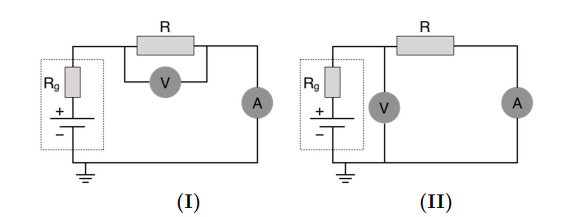
\includegraphics[width=.7\textwidth]{configurazioni.png}
    \caption{Configurazione dei circuiti.}
    \label{fig:Configurazioni_circuiti}
\end{figure}



\subsection{Misura resistenze interne Amperometro e Voltmetro}
Per trovare una stima della resistenza interna del Voltmetro è stato sufficiente applicare la legge di Ohm alla configurazione in parallelo. Abbiamo scelto una resistenza "piccola"  rispetto all'ordine di grandezza della resistenza $R_v$ del voltmetro, pari a: $$R = (302.1\pm0.1)\ \text{k}\Omega$$ il cui valore è stato misurato con un multimetro palmare e verificato con una \href{https://www.arrow.com/it-it/research-and-events/articles/resistor-color-code}{tabella dei codici colore dei resistori.}\\
Applicando al circuito con un generatore una tensione: $V = (5.000\pm0.001)$V e utilizzando un amperometro da banco per la misura della corrente abbiamo registrato $I = (17.00\pm0.01)\mu\text{A}$. Svolgendo il calcolo con la legge di Ohm: 

\begin{equation}
    V= R_{\text{eq}} \cdot I
    \label{legge di ohm}
\end{equation}

\begin{equation}
    \label{resistenza eq parallelo}
    R_{eq}= \frac{1}{\frac{1}{R_1} + \frac{1}{R_2}} = \frac{R_1 R_2}{R_1 + R_2}
\end{equation}
si trova una resistenza interna del voltmetro pari a:
\begin{equation}
    R_v= (11.1\pm0.3)\cdot10^6\ \Omega
    \label{resistenza voltmetro}
    \notag
\end{equation}
L'incertezza sulla misura della resistenza  è stata calcolata con l'opportuna formula per la propagazione degli errori tenendo conto della formula (\ref{resistenza eq parallelo})
\\
\\ Per la misura della resistenza interna dell'amperometro $R_a$  abbiamo scelto una resistenza "grande" rispetto all'ordine di grandezza, pari a: $$R= (12.9\pm0.1)\ \Omega$$
il cui valore, come in precedenza, è stato ottenuto con un multimetro palmare e verificato con una \href{https://www.arrow.com/it-it/research-and-events/articles/resistor-color-code}{tabella dei codici colore dei resistori.}
\\Applicando con un generatore una tensione pari a $V = (2.500\pm0.001)\text{V}$ e utilizzando lo stesso amperometro da banco abbiamo misurato la corrente $ I = (173.00\pm0.01) m\text{A}$. Svolgendo il calcolo con la legge di Ohm in serie: 

$$
    V= R_{eq} \cdot I
$$
\begin{equation}
    R_{eq}= R + R_a
    \label{resistenza eq serie}
\end{equation}
si trova una resistenza interna dell'amperometro pari a:

\begin{equation}
    R_a= (1.551\pm0.001)\ \Omega
    \label{resistenza amperometro}
    \notag
\end{equation}

\subsection{Verifica Legge di Ohm}
Lo scopo di questa sezione è quello di verificare in modo quantitativo la rinomata relazione lineare tra corrente e tensione data dalla legge di ohm (\ref{legge di ohm})\\
Per farlo abbiamo utilizzato la configurazione \ref{fig:Configurazioni_circuiti}  del circuito aggiungendo una resistenza il cui valore atteso è pari a: $$R_{attesa} = (1000.0\pm0.1)\ \Omega$$
La scelta della configurazione è collegata al confronto tra le resistenze interne degli strumenti di misura con la resistenza $R$ del circuito. 
Abbiamo preso ripetute misure, variando la tensione del generatore, utilizzando poi un multimetro palmare per ottenere una misura della tensione $V$ e un amperometro da banco (più preciso per correnti basse) per la misura della corrente $I$.
\\

\subsubsection{Dati legge di Ohm}
Di seguito sono riportate le misure effettuate nella Tabella \ref{tab:Misure legge Ohm}, una Tabella\ref{tab:Tab_compatib_ohm} riassuntiva per la compatibilità delle misure e il grafico \ref{fig:Fit legge ohm} del fit lineare eseguito con la libreria minuit. Per quanto riguarda gli errori:
\begin{enumerate}
\item Incertezza sulla tensione $V=(\pm0.001)$, ovvero sensibilità del multimetro palmare.
\item Incertezza sulla corrente $I$ è stata calcolata utilizzando le istruzioni sulla tabella di riferimento fornita dal produttore del multimetro \ref{fig:Tabella_sensibilità}
\end{enumerate}
\newpage

\begin{figure}[htbp]
    \centering
    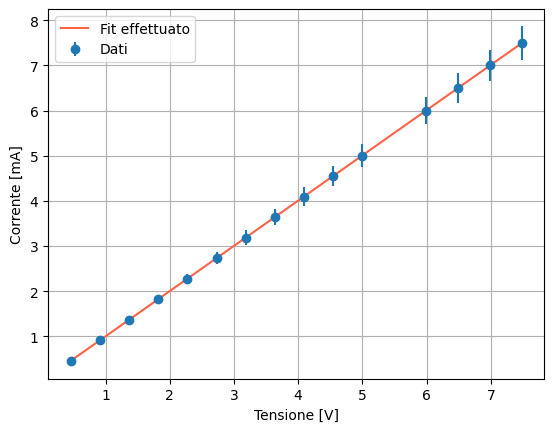
\includegraphics[width=.65\textwidth]{verifica_legge_di_ohm.png}
    \caption{Fit legge di Ohm}
    \label{fig:Fit legge ohm}
\end{figure}


\vspace{0.5cm}
A partire dall'interpolazione abbiamo estratto il valore della resistenza $R$ invertendo il coefficiente angolare della retta e propagando l'errore. Abbiamo trovato come valore di resistenza:
$$ R_{\text{misurata}} = (998\pm18)\ \Omega \quad R_{\text{attesa}} = (1000.0\pm0.1)\ \Omega$$


\subsubsection{Conclusioni verifica legge di Ohm}
Analizzando il risultato dell'interpolazione dei dati possiamo affermare che il test del $\chi^2$ conferma la validità della legge di Ohm. La forma funzionale utilizzata per il fit è: $$y=mx+q$$
La leggera discrepanza tra il valore misurato della resistenza e il valore atteso rientra in un range accettabile per questo contesto sperimentale, infatti la differenza percentuale tra valore misurato e atteso è del $0.2\%$. Il fit è stato eseguito utilizzando le librerie iminuit e le opportune funzioni per regressioni lineari. I risultati restituiti per la validità sono:
\begin{enumerate}
    \item $\chi^2 = 0.0008$
    \item $p-value \approx 1.0$
\end{enumerate}
Questi risultati forniscono ulteriore confidenza sulla coerenza dei dati con il modello della legge di Ohm.



\subsection{Resistenze Composite}
Un'ulteriore verifica della legge di ohm è stata fatta applicando le nozioni di teoria sulle \textbf{resistenze composite.} In questa parte dell'esperienza l'obiettivo è quello di misurare valori di correnti e tensione in due configurazioni di circuiti: la prima con resistenze in serie e la seconda con resistenze in parallelo, tenendo conto di scegliere resistenze con valori simili (ordine di grandezza).



\subsection{Resistenze in serie}
Ci aspettiamo che le resistenze in serie si compongano secondo la legge (\ref{resistenza eq serie})\\
Le resistenze scelte sono: $$R_1 = (149.0\pm0.1)\  k\Omega$$
$$R_2 = (100.0\pm0.1)\  k\Omega$$
Per gli errori sulle misure abbiamo preso le seguenti considerazioni: 
\begin{enumerate}
\item Incertezza sulla tensione $V=(\pm0,001)$, ovvero sensibilità del multimetro palmare
\item Incertezza sulla corrente $I$ è stata calcolata di nuovo utilizzando le istruzioni sulla tabella di riferimento fornita dal produttore del multimetro \ref{fig:Tabella_sensibilità}
\end{enumerate}
\vspace{20pt}
Invertendo il valore del coefficiente angolare e propagando l'errore dell'interpolazione, abbiamo ricavato il valore della resistenza :

\begin{equation}
     R_{attesa}= (249.0 \pm0.1) k\Omega \qquad  R_{ misurata} = (243.4 \pm 6.2) k\Omega
    \label{resistenza serie}
    \notag
\end{equation}

\subsection{Resistenze in parallelo}
Dalla teoria sappiamo che le resistenze in parallelo si compongono con la formula \eqref{resistenza eq parallelo}.\\
Le resistenze scelte per la verifica sono: $$R_1 = (149.0\pm0.1)\ k\Omega$$
$$R_2 = (100.0\pm0.1)\  k\Omega$$\\
Per gli errori sulle misure abbiamo preso le seguenti indicazioni: 
\begin{enumerate}
\item Incertezza sulla tensione $V=(\pm0,001)$, ovvero sensibilità del multimetro palmare
\item Incertezza sulla corrente $I$ è stata calcolata allo stesso modo utilizzando come in precedenza le istruzioni sulla tabella di riferimento fornita dal produttore del multimetro \ref{fig:Tabella_sensibilità}
\end{enumerate}
Invertendo il valore del coefficiente angolare e propagando l'errore dell'interpolazione, abbiamo ricavato il valore della resistenza equivalente:

\begin{equation}
     R_{attesa}= (46.2 \pm0.5)\ k\Omega \qquad  R_{ misurata} = (46.1 \pm 1.1)\ k\Omega
    \label{resistenza parallelo}
    \notag
\end{equation}

\begin{figure}[htbp]
    \centering
    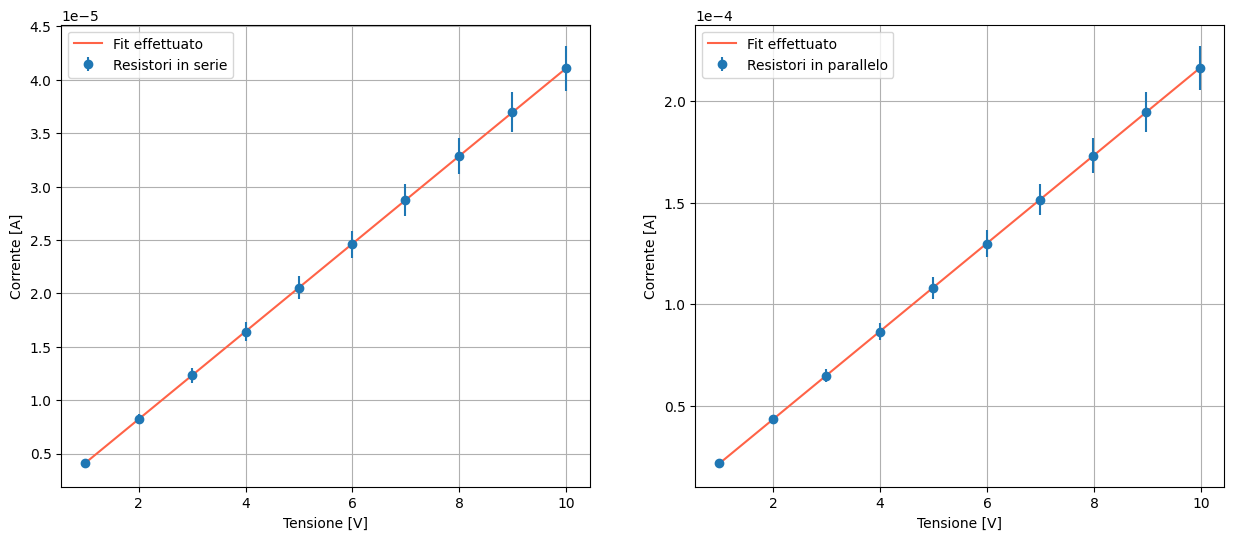
\includegraphics[width=.65\textwidth]{fit_resistenze_composite.png}
    \caption{Fit dei dati raccolti dalle resistenze composite: a sinistra in serie, a destra in parallelo}
    \label{fig:Fit resistenze composite}
\end{figure}


\subsubsection{Conclusioni dati resistenze composite}
Per quanto riguarda le misure prese sulle resistenze in serie, analizzando il grafico e i risultati del fit con il medesimo modello lineare: $y=mx+q$ è evidente la coerenza dei dati misurati.\\
In questo caso la differenza percentuale tra $R_{attesa}$ e $R_{misurata}$ è pari a $2.25\%$, di nuovo un risultato accettabile per questo contesto.
Il test del $\chi^2$ eseguito ha restituito i seguenti valori: 
\begin{enumerate}
    \item $\chi^2 = 0.006$
    \item $p-value \approx 1.0$
\end{enumerate}
Valori che confermano la coerenza dei dati misurati con la legge per le resistenze in serie.
Per le misure prese sulle resistenze in parallelo, di nuovo è evidente la validità della legge lineare, analizzando il grafico e in particolare il test del $\chi^2$ otteniamo:
\begin{enumerate}
    \item $\chi^2 = 0.0013$
    \item $p-value \approx 1.0$
\end{enumerate}
In questo caso delle resistenze in parallelo la differenza percentuale tra la $R_{misurata}$ e $R_{attesa}$ è pari al $0.22\%$.
La leggera differenza di precisione dei risultati ottenuti per i due casi separati di resistenze in serie e in parallelo è sufficientemente bassa da essere collegata a normali variazioni stocastiche nel processo di misurazione.
Tutti questi risultati indicano una forte coerenza tra il modello lineare e i dati misurati.
\section{Partitore Resistivo}

\subsection{Accenno alle Leggi di Kirchhoff}
Per aiutarci nella risoluzione dei circuiti, possiamo fare affidamento alle leggi di Kirchhoff:
\begin{enumerate}
    \item \textbf{Legge dei nodi}: la somma algebrica delle correnti che attraversano un nodo (con segno diverso se entranti o uscenti) è nulla.
    \item \textbf{Legge delle maglie}: la somma algebrica delle cadute di potenziale in una maglia chiusa è uguale a zero.
\end{enumerate}

\subsection{Considerazioni Teoriche}
\begin{figure}
    \centering
    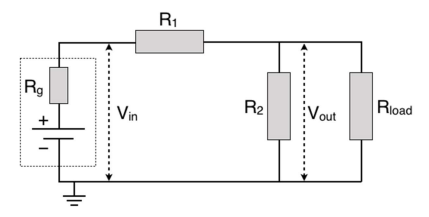
\includegraphics[width=.7\textwidth]{partitore_resistivo.png}
    \caption{Schema del partitore resistivo}
    \label{fig:partitore resistivo}
\end{figure}

Facendo uso delle due leggi sopra elencate, possiamo osservare la figura \ref{fig:partitore resistivo} e domandarci quali debbano essere $R_1 \text{ e } R_2$ affinché: $$V_{out} = \frac{1}{2}V_{in}$$.\\
Dalla legge delle maglie possiamo ricavare:
\begin{align*}
    V_{in} &- V_1 - V_{out} = 0 \\
    V_{in} &= V_1 + V_{out}
\end{align*}
Dal momento che $V_{out} = \frac{1}{2}V_{in}$, si ottiene che:
$$
    V_{in} = V_1 + \frac{1}{2}V_{in} \implies V_1 = V_{out} = \frac{1}{2}V_{in} \\
$$\\
Ricorrendo alla legge di Ohm, possiamo dividere entrambi i membri per $I$ e ottenere la resistenza associata ad ogni tensione.\\
Inoltre, essendo $V_{in}$ la differenza di potenziale ai capi del generatore, segue la legge $$V_{in} = R_{tot} \cdot I$$ 
dove $R_{tot}$ rappresenta la resistenza totale del circuito (avendo assunto $R_g \approx 0$)
\begin{align*}
    \frac{V_{in}}{I} &= \frac{V_1}{I} + \frac{V_{out}}{I}\\
    \vspace{10pt}
    R_{tot} &= R_1 + R_2
\end{align*} \\
Siccome $V_1 = V_{out}$, allora si trova:
$$R_1 = R_2$$
Per ottenere questo risultato non abbiamo tenuto conto della presenza di $R_{load}$, tuttavia si dimostra facilmente che tale valore risulta trascurabile.\\
Infatti, chiamando $R_{out}$ la resistenza equivalente a $R_2$ e $R_{load}$ in parallelo:
$$
\frac{1}{R_{out}} = \frac{1}{R_2} + \frac{1}{R_{load}}
$$
Nel caso in cui $R_{load} >> R_2$
$$
\frac{1}{R_{out}} \approx \frac{1}{R_2} \implies R_{out} \approx R_2
$$
Dunque,$V_{out}$ non dipende da $R_{load}$, abbiamo inoltre effettuato alcune misure per verificare tale risultato, riportate nella tabella \ref{tab:Misura tensione Rload}

\section{Misure corrente-tensione Diodo}
In quest'ultima parte dell'esperienza l'obiettivo è lo studio della relazione tensione-corrente in un circuito composto da un generatore e un diodo, in particolare lo scopo era di:

\begin{enumerate}
    \item Verificare la legge di Shockley:
        \begin{equation}
            I = I_0(e^{\frac{qV}{gkT}}-1)
            \label{legge di Shockley}
        \end{equation}
     Dove $I_0$ è la corrente di saturazione inversa, $q$ è la carica dell'elettrone , $V$ è la tensione, $g$ è una costante adimensionale tipica del diodo, $k$ è la costante di Boltzmann e $T$è la temperatura.
    \item Valutare la tensione di soglia $V_{soglia}$, ovvero il valore della tensione oltre al quale il diodo inzia a condurre.
\end{enumerate}
Abbiamo registrato le misure al variare della tensione di alimentazione in un range da $0$ a $\SI{500}{\milli\ampere}$, misurando la differenza di potenziale ai capi del diodo e la corrente che lo attraversa. Abbiamo scelto la configurazione \ref{fig:Configurazioni_circuiti} del circuito, avendo cura di accertarci che per tutti i valori di corrente e tensione presi in esame, la resistenza del diodo non aumentasse al punto da dover scegliere la seconda configurazione.

\subsection{Dati raccolti per diodo}
Di seguito abbiamo riportato le misure per tensione, corrente e incertezza sulla corrente effettuate per il circuito con il diodo. Tali misure sono riportate in una tabella a fine della relazione.
\ref{tab:Misure diodo}:

\subsection{Fit con legge di Shockley}
Riportati in figura \ref{fig:Dati raccolti e fit lineare Shockley} ci sono i dati raccolti elencati nella tabella \ref{tab:Misure diodo}, rappresentati in blu. In rosso è disegnata l'interpolazione della legge di Shockley \ref{legge di Shockley}: 
%$$
%I = I_0(e^{\frac{qV}{gkT}}-1)
%$$
\begin{figure}[h!]
    \centering
    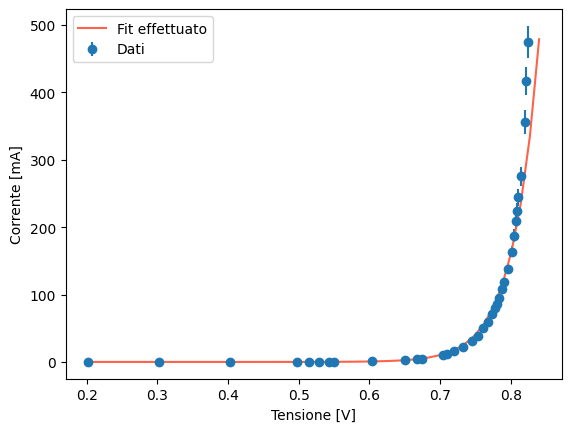
\includegraphics[width=.8\textwidth]{legge_shockley.png}
    \caption{Dati raccolti e fit della legge di Shockley.}
    \label{fig:Dati raccolti e fit lineare Shockley}
\end{figure}
Per verificare la validità dei dati abbiamo svolto un test del $\chi^{2}$ restituendo un valore pari a: $$\widetilde{\chi}^2= 8.9$$ 
A partire dall'interpolazione svolta con la libreria iminuit abbiamo estratto i valori d'interesse di $I_0$ e $g$, ottenendo:
\begin{enumerate}
    \item $I_0 = (47\pm3)\ nA$
    \item $g = (1.407\pm0.004)$
\end{enumerate}
Osservando il valore del $\widetilde{\chi}^2$ abbiamo deciso di rappresentare il grafico dei residui, in modo tale da analizzare la situazione, riportiamo in figura \ref{fig:residui_shockley} tale grafico.

\begin{figure}[h!]
    \centering
    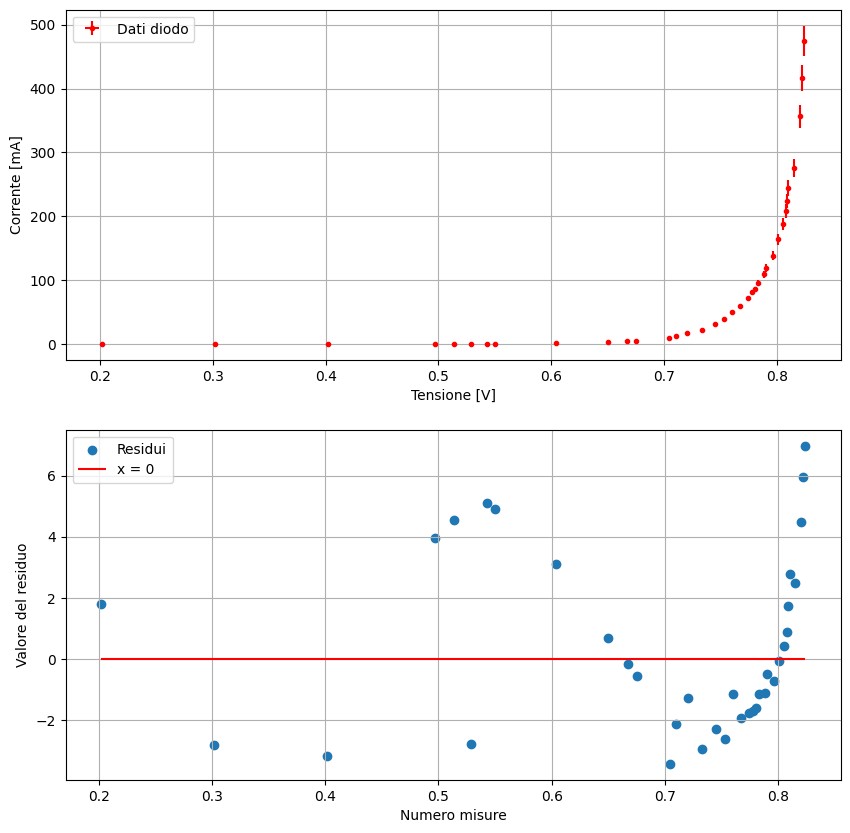
\includegraphics[width=.8\textwidth]{Residui.png}
    \caption{Grafico dei residui per l'interpolazione della legge di Shockley.}
    \label{fig:residui_shockley}
\end{figure}
\newpage
\vspace{40pt}
\subsubsection{Conclusioni su fit e grafico resuidi per diodo}


E' possibile notare una crescita netta dei residui dalla misura 19 in poi. Avendo calcolato i residui come:
$$
R = \frac{I_{misurato} - I_{atteso}}{\sigma_{stimata}}
$$
il loro aumento implica un aumento di $I_{misurato}$. Abbiamo provato a spiegare questa osservazione con un cambiamento graduale della temperatura del diodo, in quanto la corrente condotta dipende esponenzialmente dall'inverso della temperatura. Per questo motivo, un piccolo cambiamento di $T$ corrisponde ad effetti significativi sulla corrente trasmessa. \\
Tale conclusione è abbastanza ragionevole dato che il diodo è noto per essere un componente fortemente influenzato dalla temperatura. 
Per motivare qualitativamente questa osservazione abbiamo anche a fisicamente cambiare la temperatura, provando a soffiare e stringere in mano il diodo durante una misurazione e abbiamo notato che la lettura della corrente cominciava effettivamente ad oscillare.

\newpage

\subsection{Tensione soglia}
L'obiettivo di quest'ultima parte,come già detto precedentemente, è quello di ricavare una \textbf{stima della tensione di soglia} del diodo in analisi. Per tensione di soglia si intende il valore minimo di tensione applicabile ai capi del diodo affinché esso inizi a condurre una quantità significativa di corrente (nel caso più generale $\sim$ \SI{10}{\milli\ampere}).
Per trovare il valore di tensione $V_{soglia}$ abbiamo interpolato gli ultimi dati raccolti con una retta, finché il valore del $\chi^{2}$ non è rimasto paragonabile a $\sim$1. Intersecando la retta con l'asse orizzontale si ricava il valore della tensione soglia. Come migliore stima abbiamo ottenuto: 
\begin{equation}
    V_{soglia} = (0,7\pm0,1) V
    \label{tensione soglia}
    \notag
\end{equation}
Riportiamo in figura \ref{fig:tensione soglia} il fit lineare delle ultime misure raccolte utilizzato per stimare $V_{soglia}$.

\begin{figure}[htbp]
    \centering
    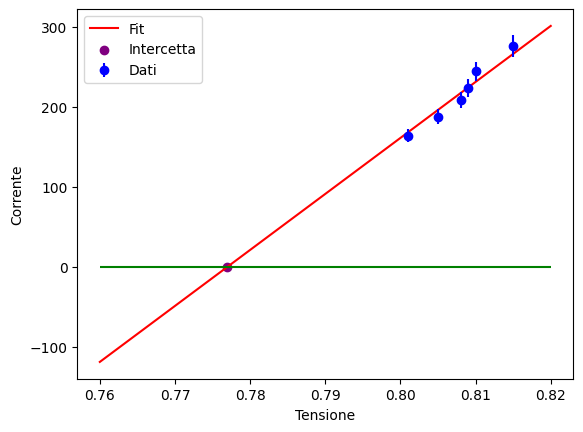
\includegraphics[width=.7\textwidth]{tensioni_alte_shockley.png}
    \caption{Fit lineare per tensioni alte.}
    \label{fig:tensione soglia}
\end{figure}

\newpage
\subsection{Considerazioni finali}
In questa sezione, riassumiamo le conclusioni emerse dall'esperienza e valutiamo la coerenza dei risultati ottenuti rispetto ai valori attesi, oltre ad esaminare i test utilizzati per verificarli. Il documento completo dell'analisi dei dati è disponibile al seguente \href{https://colab.research.google.com/drive/184wsEQVv36AxDK5J4vkgR3OajIU9M9VG?usp=sharing}{link}


\subsection{Conclusioni prima parte: Legge di Ohm}
La domanda che ci era stata posta inizialmente per questa parte dell'esperienza era: 
$$\text{Quale è la configurazione di circuito più adatta? \ref{fig:Configurazioni_circuiti}}$$ 
Inizialmente è stato quindi necessario stimare le resistenze "parassite" dei dispositivi di misura:
\renewcommand{\labelitemi}{-}
\begin{enumerate}
    \item Nella configurazione I con il Voltmetro in parallelo è necessario usare $R$ "grandi" al fine di minimizzare il flusso di corrente che attraversa il Voltmetro stesso
    \item Nella configurazione II con l'amperometro in serie è necessario usare $R$ "piccole" in modo tale da far fluire più corrente possibile all'Amperometro
\end{enumerate}
Quello che abbiamo ottenuto da queste verifiche sperimentali è che al fine di minimizzare la perturbazione delle misure di grandezze come corrente e tensione di un circuito la cosa più importante da fare è regolare i valori delle resistenze. 


\subsubsection{Effetto resistenza parassite}
E' possibile valutare quantitativamente l'effetto delle resistenze interne dei Multimetri considerando la teoria delle \textbf{leggi di Kirchhoff}. Si può calcolare l'errore introdotto dalle resistenze interne e successivamente confrontarlo con l'errore sui valori misurati. Se l'errore introdotto dalle resistenze interne è compatibili con l'errore accettabile allora trascurare l'effetto introdotto dai multimetri.
Di seguito viene riportato un esempio di questo calcolo.\\
La formula per calcolare la tensione effettiva:
\begin{equation}
    V_{eff}= \frac{V_m}{1+\frac{R_v}{R}}
    \label{Tensione considerando R interna voltmetro}
\end{equation}
dove:
\begin{itemize}
    \item $V_m$ è la tensione misurata dal voltmetro
    \item $R$ è la resistenza reale del circuito 
    \item $R_v$ è la resistenza del voltmetro 
\end{itemize}
se consideriamo la resistenza interna del voltmetro pari a $R_v=(11.1\pm0.3) M\Omega$, con casi estremi:
\begin{itemize}
    \item $R_V = \SI{11.4}{\mega\ohm}$ massimo errore positivo
    \item $R_v = \SI{10.8}{\mega\ohm}$ massimo errore negativo
\end{itemize}
Come incertezza  sulla tensione prendiamo $(\pm0.001)V$ per ogni misura effettuata calcoliamo $V_\text{eff}$ in entrambi i casi estremi di resistenza del voltmetro. 
Ad esempio prendendo una misura:
\begin{itemize}
    \item $V_m = \SI{0.457}{\volt}$
    \item $I = \SI{0.46}{\milli\ampere}$
    \item $I_\text{err}=\SI{0.02}{\milli\ampere} $
\end{itemize}
Calcolando la tensione effettiva per i due casi estremi otteniamo:
\begin{itemize}
    \item \( V_\text{eff+}= \dfrac{0.457}{1+\dfrac{11.4 \times 10^{-6}}{1000}} \)
    \item \( V_\text{eff-}= \dfrac{0.457}{1+\dfrac{10.8 \times 10^{-6}}{1000}} \)
\end{itemize}
Successivamente calcoliamo l'errore assoluto tra $V$ e $V_\text{eff}$ per entrambi i casi:
\begin{itemize}
    \item Errore+ = $|0.4570 - 0.4569| \sim 0.0001$
    \item Errore- = $|0.4570 - 0.4569| \sim 0.0001$
\end{itemize}
Come si può notare l'errore è assolutamente trascurabile essendo pari a $\pm(0.0001)$ molto minore rispetto all'errore riferito alla tensione $(\pm0.001)$.
\\


\subsection{Conclusioni seconda parte: Potenza e partitore resistivo}
Per confermare i calcoli teorici svolti abbiamo deciso di utilizzare due resistenze di pari valore e misurare la differenza di potenziale ai capi di $R_{load}$. Abbiamo  osservato che, al crescere di $R_{load}$, la tensione $V_{out}$ aumentava fino a stabilizzarsi rapidamente attorno alla metà del valore di tensione $V_{in}$. Abbiamo riportato i dati raccolti nella tabella:

\subsection{Conclusioni terza parte: Diodo}
\subsubsection{Misurazione $I_0$, $g$}
In conclusione, i valori estratti per $I_0$ e $g$ sono coerenti con le aspettative teoriche della legge di Shockley. Tuttavia, l'analisi dei residui suggerisce l'importanza di considerare gli effetti della temperatura nelle misurazioni del diodo, poiché anche variazioni minime possono influenzare significativamente i risultati sperimentali.

\subsubsection{Misurazione tensione di soglia}
 Eseguendo la regressione lineare sulle ultime sei misure abbiamo ottenuto il valore della tensione di soglia intersecando la retta con l'asse x, selezionando punti a partire dall'ultimo fino a quando il $\chi^2$ non superava 1. \ref{tensione soglia}.

\newpage    
\subsection{Tabelle dati} 

\begin{table}[h!]
    \begin{subtable}{0.5\textwidth}
        \centering
        \begin{tabular}{ccc}
            \toprule
            \rowcolor{blue!10}
            \textbf{$V[V]$} & \textbf{$I[\mu A]$} & \textbf{$I_{\text{err}}[\mu A]$} \\
            \midrule
            0.457 & 460 & 20 \\
            0.911 & 910 & 50 \\
            1.365 & 1370 & 70 \\
            1.820 & 1820 & 90 \\
            2.274 & 2300 & 100 \\
            2.729 & 2700 & 100 \\
            3.183 & 3200 & 200 \\
            3.637 & 3600 & 200 \\
            4.091 & 4100 & 200 \\
            4.546 & 4600 & 200 \\
            5.000 & 5000 & 300 \\
            5.993 & 6000 & 300 \\
            6.492 & 6500 & 300 \\
            6.990 & 7000 & 400 \\
            7.480 & 7500 & 400 \\
            \bottomrule
        \end{tabular}
        \captionsetup{position=bottom}
        \caption{Misure legge di Ohm}
        \label{tab:Misure legge Ohm}
    \end{subtable}%
    \begin{subtable}{0.5\textwidth}
        \centering
        \begin{tabular}{c|c}
            \hline
            \cellcolor{blue!10}$\chi^2$ & $0.00086$ \\ \hline
            \cellcolor{blue!10}p-value & $1.00$ \\ \hline
            \cellcolor{blue!10}t-test& $0.8$ $\sigma$ \\
            \hline
        \end{tabular}
        \caption{Tabella compatibilità fit Ohm.}
        \label{tab:Tab_compatib_ohm}
    \end{subtable}
\end{table} 

\begin{table}[htbp]
\begin{subtable}{0.5\textwidth}
    \centering
    \begin{tabular}{ccc}
        \toprule
        \rowcolor{blue!10}
    \textbf{$V$[V]}  & \textbf{$I$[mA]}   & \textbf{$I_{err}$[mA]} \\
        \midrule
        1,000 & 22    & 1        \\
        1,998 & 43    & 2        \\
        2,996 & 65    & 3        \\
        3,994 & 87    & 4        \\
        4,991 & 108   & 5        \\
        5,989 & 130   & 7        \\
        6,990 & 152   & 8        \\
        7,980 & 173   & 9        \\
        8,970 & 195   & 10       \\
        9,970 & 216   & 11       \\
        \bottomrule
    \end{tabular}
    \caption{Misure resistenze in parallelo}
    \label{subtab:Misure_ohm_R_parallelo}
\end{subtable}
\begin{subtable}{0.5\textwidth}
    \centering
    \begin{tabular}{c|c}
    \hline
    \cellcolor{blue!10}$\chi^2$ & 0.0013 \\ \hline
    \cellcolor{blue!10}p-value & 0.99 \\ \hline
    \cellcolor{blue!10}t-test & 0.1 \\ \hline
\end{tabular}
\caption{Tabella compatibilità R parallelo.}
\label{subtab:Tab_compatib_ohm_parallelo}
\notag
\end{subtable}
\end{table}

\begin{table}[htbp]
\begin{subtable}{0.5\textwidth}
    \centering
    \begin{tabular}{ccc}
        \toprule
        \rowcolor{blue!10}
    \textbf{$V$[V]} & \textbf{$I$ [mA]}   & \textbf{$I_{err}$[mA]} \\
        \midrule
        1,002 & 4,12  & 0,26 \\ 
        2,002 & 8,22  & 0,46 \\ 
        3,001 & 12,32 & 0,67 \\ 
        4,001 & 16,41 & 0,87 \\ 
        5,001 & 20,51 & 1,08 \\ 
        6,001 & 24,60  & 1,28 \\ 
        6,990 & 28,77 & 1,49 \\ 
        7,990 & 32,87 & 1,69 \\ 
        8,990 & 36,98 & 1,90  \\ 
        9,990 & 41,09 & 2,10  \\ 
        \bottomrule
    \end{tabular}
    \caption{Misure Resistenze in serie}
    \label{subtab:Misure_ohm_R_serie}
\end{subtable}%
\begin{subtable}{0.5\textwidth}
\centering
\begin{tabular}{c|c}
    \hline
    \cellcolor{blue!10}$\chi^2$ & $0.0068$ \\ \hline
    \cellcolor{blue!10}p-value & $0.99$ \\ \hline
    \cellcolor{blue!10}t-test & $0.9$ \\
    \hline
    \end{tabular}
    \caption{Tabella compatibilità R in serie.}
    \label{subtab:Tab_compatib_ohm_serie}
    \end{subtable}
\end{table}

\begin{table}[htbp]
\centering
\begin{tabular}{c|c}
    \toprule
    \rowcolor{blue!10}
    $R_{load}$ [$k\Omega$] & $V_{out}$ [V]\\
    \hline
    0.01 & 0.028\\
    0.50 & 0.490\\
    10 & 51.00\\
    500 & 51.00\\
    1000 & 51.00\\
    \hline
    \end{tabular}
    \caption{Misura della tensione al variare di $R_{load}$}
    \label{tab:Misura tensione Rload}
\end{table}

\begin{table}[htbp]
\centering
\rowcolors{2}{blue!10}{white} % Alternate row colors starting from the second row
\begin{tabular}{ccc}
    \toprule
    \textbf{$V$ [V]} & \textbf{$I$ [mA]} & \textbf{$I_{\text{err}}$ [mA]} \\
    \midrule
    0.202 & 0.00003 & 0.00001 \\
    0.302 & 0.00013 & 0.00002 \\
    0.402 & 0.0024 & 0.0002 \\
    0.497 & 0.049 & 0.002 \\
    0.514 & 0.081 & 0.004 \\
    0.529 & 0.083 & 0.004 \\
    0.543 & 0.187 & 0.009 \\
    0.550 & 0.22 & 0.01 \\
    0.604 & 0.88 & 0.04 \\
    0.650 & 2.7 & 0.1 \\
    0.667 & 4.1 & 0.2 \\
    0.675 & 5.0 & 0.3 \\
    0.704 & 9.8 & 0.5 \\
    0.710 & 12.2 & 0.6 \\
    0.720 & 16.7 & 0.8 \\
    0.733 & 22 & 1 \\
    0.745 & 32 & 2 \\
    0.753 & 39 & 2 \\
    0.760 & 50 & 3 \\
    0.767 & 59 & 3 \\
    0.774 & 72 & 4 \\
    0.778 & 81 & 4 \\
    0.780 & 85 & 4 \\
    0.783 & 95 & 5 \\
    0.788 & 109 & 5 \\
    0.790 & 119 & 6 \\
    0.796 & 138 & 7 \\
    0.801 & 164 & 8 \\
    0.805 & 187 & 9 \\
    0.808 & 208 & 10 \\
    0.809 & 224 & 11 \\
    0.810 & 244 & 12 \\
    0.815 & 275 & 14 \\
    0.820 & 357 & 18 \\
    0.822 & 417 & 21 \\
    0.824 & 475 & 24 \\
    \bottomrule
\end{tabular}
\caption{Misure corrente-tensione per diodo}
\label{tab:Misure diodo}
\end{table}



\begin{figure}[h!] % questa la sposterei alla fine
    \centering
    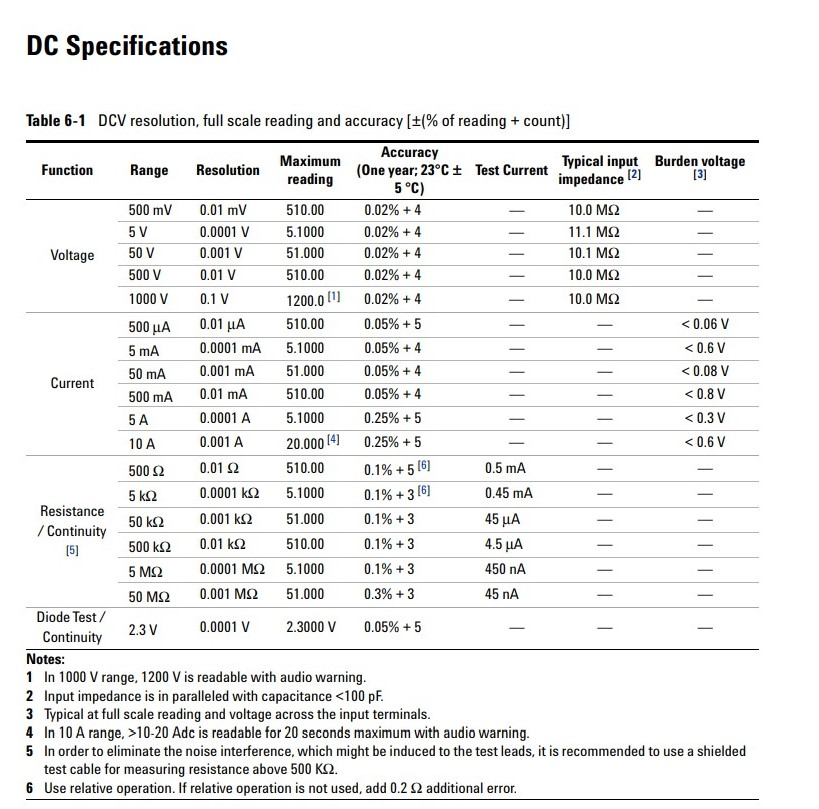
\includegraphics[width=1\textwidth]{tabella_errori.png}
    \caption{Tabella sulla sensibilità fornitore multimetro.}
    \label{fig:Tabella_sensibilità}
\end{figure}


\end{document}
